\documentclass{article}
\usepackage[utf8]{inputenc}
\usepackage{graphicx}
\usepackage{listings}
\usepackage{xcolor}
\definecolor{codegreen}{rgb}{0,0.6,0}
\definecolor{codegray}{rgb}{0.5,0.5,0.5}
\definecolor{codepurple}{rgb}{0.58,0,0.82}
\definecolor{backcolour}{rgb}{0.95,0.95,0.92}
\lstdefinestyle{mystyle}{
    backgroundcolor=\color{backcolour},   
    commentstyle=\color{codegreen},
    keywordstyle=\color{magenta},
    numberstyle=\tiny\color{codegray},
    stringstyle=\color{codepurple},
    basicstyle=\ttfamily\footnotesize,
    breakatwhitespace=false,         
    breaklines=true,                 
    captionpos=b,                    
    keepspaces=true,                 
    numbers=left,                    
    numbersep=5pt,                  
    showspaces=false,                
    showstringspaces=false,
    showtabs=false,                  
    tabsize=2
}
\lstset{style=mystyle}
\graphicspath{{./presentation_figures/}}

\title{MLPR 2019 - Assignment 1}
\author{Vasilis Gkolemis, Sokratis Lyras}

\date{October 2019}

\begin{document}

\maketitle

\section{Question 1}
\subsection{Question 1a}

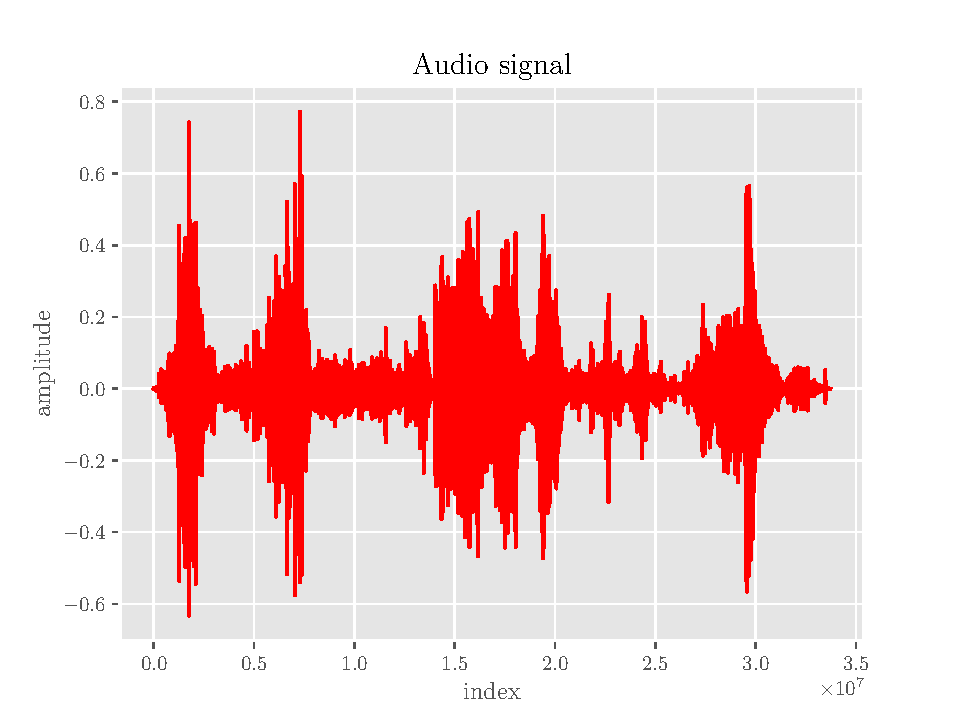
\includegraphics[scale=0.75]{fig_01.pdf}

We observe that the distribution of amplitudes varies among the different parts of the song. This is a frequent phenomenon in audio signals.

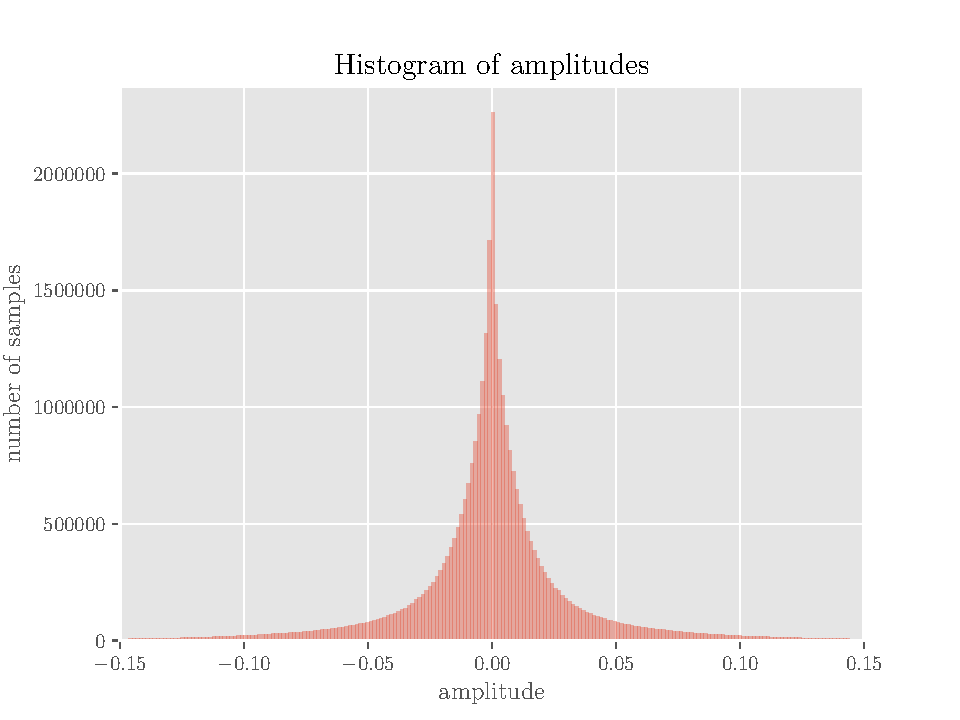
\includegraphics[scale=0.75]{fig_02.pdf}

We observe that the distribution of amplitudes along the whole song is zero centered. The distribution, although attenuates exponentially as we move away from the center, is \textbf{not} a gaussian distribution.

\subsection{Question 1b}

The code snippet that creates the dataset:

\begin{lstlisting}[language=Python]
class Dataset:
    amp_data = amp_data
    
    def __init__(self, D: int, split_pcg = [0.7, 0.15, 0.15]):
        """
        
        :param D: dimensionality 
        """
        
        # rearrange signal into non-overlapping arrays of shape [N x D+1]
        self.remaining_samples = amp_data.shape[0] % (D+1)
        self.XY = amp_data[:-self.remaining_samples] if self.remaining_samples > 0 else amp_data
        self.XY = self.XY.reshape((int(self.XY.shape[0]/(D+1)), (D+1)))
        
        # shuffle (not inplace)
        self.shuffle_indices = np.random.permutation(self.XY.shape[0])
        self.XY_shuffled = np.take(self.XY, self.shuffle_indices, axis=0)
        
        # split into training
        self.nof_tr = np.int(np.floor(self.XY.shape[0] * split_pcg[0]))
        self.nof_val = np.int(np.floor(self.XY.shape[0] * split_pcg[1]))
        self.nof_test = np.int(np.floor(self.XY.shape[0] * split_pcg[2]))
        
        train_start = 0
        val_start = self.nof_tr
        test_start = self.nof_tr + self.nof_val
        
        self.X_shuf_train = self.XY_shuffled[0 : self.nof_tr, :D]
        self.y_shuf_train = self.XY_shuffled[0 : self.nof_tr, D]
        
        self.X_shuf_val = self.XY_shuffled[val_start : val_start + self.nof_val, :D]
        self.y_shuf_val = self.XY_shuffled[val_start : val_start + self.nof_val, D]
        
        self.X_shuf_test = self.XY_shuffled[test_start : test_start + self.nof_test, :D]
        self.y_shuf_test = self.XY_shuffled[test_start : test_start + self.nof_test, D]
    
D = 20
split_pcg = [0.7, 0.15, 0.15]
data = Dataset(D, split_pcg)
\end{lstlisting}

%%%%%%%%%%%%%%%%%%%%%%%%%%%%%%%%%%%%%%%%%%%%%%%%%%%%%%%%%%
\section{Question 2}
\subsection{Question 2a}

We randomly pick on trainingg row $(=1000)$ from our training set. We fit a linear and a quartic model on those 20 points. The models are presented in the graph below:

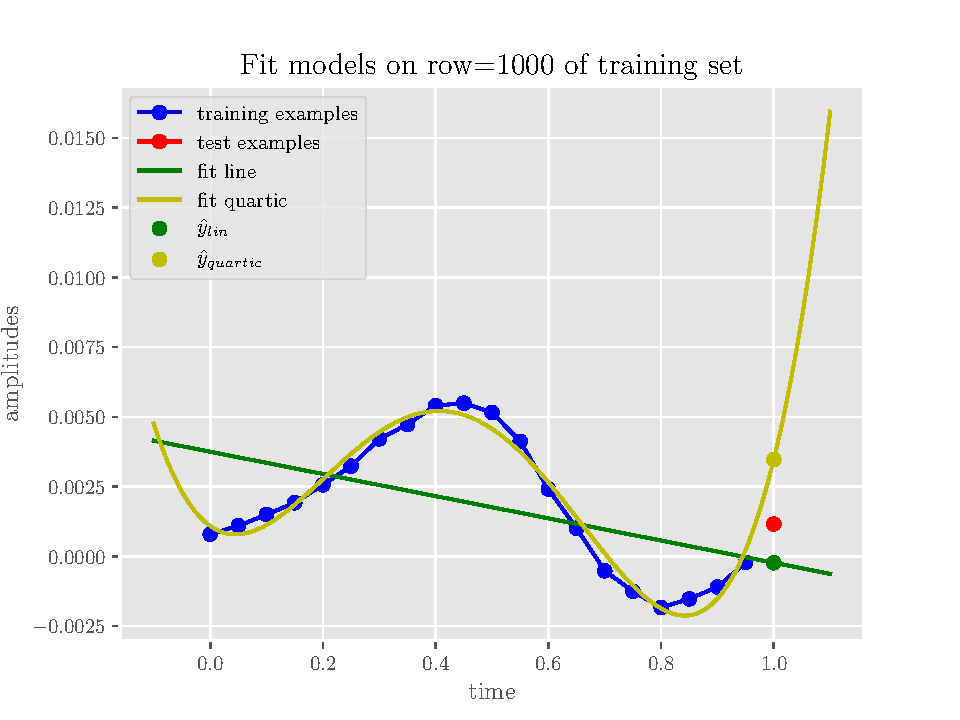
\includegraphics[scale=0.75]{fig_03.pdf}

The code snippet that fits the models and plots the graph:

\begin{lstlisting}[language = Python]
class Model:
    def __init__(self, phi):
        self.phi = phi
        self.w = None
        
    def fit(self, x: np.array, y: np.array):
        '''
        x: NxD
        y: Nx1
        
        w : Kx1
        '''
        assert len(y.shape) == 2
        assert len(x.shape) == 2
        assert x.shape[0] == y.shape[0]
        
        phi_x = self.phi(x)
        assert len(phi_x.shape) == 2
        assert phi_x.shape[0] == x.shape[0]
        
        w, residuals, rank, sv = np.linalg.lstsq(phi_x, y, rcond=None)
        self.w = w
        self.residuals = residuals
        
        assert len(self.w.shape) == 2
        assert self.w.shape[0] == phi_x.shape[1]
        assert self.w.shape[1] == 1
        return w
    
    def predict(self, x: np.array):
        '''
        x : NxD
        
        Nx1
        '''
        assert len(x.shape) == 2
        phi_x = self.phi(x)
        assert len(phi_x.shape) == 2
        assert phi_x.shape[0] == x.shape[0]
        assert phi_x.shape[1] == self.w.shape[0]
        
        return np.matmul(phi_x, self.w)
    
    
    def mse(self, X, Y):
        '''
        X : NxD
        Y : Nx1
        
        scalar
        '''
        assert len(X.shape) == 2
        assert len(Y.shape) == 2
        assert Y.shape[1] == 1
        assert X.shape[0] == Y.shape[0]
        
        Y_pred = self.predict(X)
        Y_pred.shape
        assert Y_pred.shape == Y.shape
        return np.mean(np.square(Y - Y_pred))
    
    def mae(self, X, Y):
        '''
        X : NxD
        Y : Nx1
        
        scalar
        '''
        assert len(X.shape) == 2
        assert len(Y.shape) == 2
        assert Y.shape[1] == 1
        assert X.shape[0] == Y.shape[0]
        
        Y_pred = self.predict(X)
        assert Y_pred.shape == Y.shape
        return np.mean(np.abs(Y - Y_pred))

def affine_phi(x):
    assert len(x.shape) == 2
    phi_x = np.concatenate((np.ones_like(x), x), axis=1)
    return phi_x

def quartic_phi(x):
    assert len(x.shape) == 2
    phi_x = np.concatenate((np.ones_like(x), x, x**2, x**3, x**4), axis=1)
    return phi_x


linear_model = Model(phi=affine_phi)
quartic_model = Model(phi=quartic_phi)

i = 1000 # nof row
x = np.expand_dims(np.linspace(0, 19 / 20, 20), -1)
y = np.expand_dims(data.X_shuf_train[i], -1)

linear_model.fit(x, y)
quartic_model.fit(x, y)

x_ext = np.expand_dims(np.linspace(-0.1, 1.1, 200), -1)

# subquestion a
plt.figure()

# training points
plt.plot(x, y, 'b-o', label = 'training examples')
# test point
plt.plot(np.array([[1]]), data.y_shuf_train[i], 'r-o', label = 'test examples')

# fit line
plt.plot(x_ext, linear_model.predict(x_ext), 'g-', label = 'fit line')
# fit quartic
plt.plot(x_ext, quartic_model.predict(x_ext), 'y-', label = 'fit quartic')

# prediction of linear model
plt.plot(np.array([[1]]), linear_model.predict(np.array([[1]])), 'go', label = '$\hat{y}_{lin}$')
# prediction of quartic model
plt.plot(np.array([[1]]), quartic_model.predict(np.array([[1]])), 'yo', label = '$\hat{y}_{quartic}$')

plt.xlabel("time")
plt.ylabel("amplitudes")
plt.legend();
save_filename_png = os.path.abspath("./presentation/presentation_figures/fig_03.pdf")
plt.savefig(save_filename_png)
plt.show(block=False)

\end{lstlisting}

\subsection{Qusetion 2b}
This might happen due to the much dependency of the two most recent points compared to the previous ones.In order to fit the best line for all the points, we take consideration of all points’ errors, where in this case of amplitudes this is not the case. The slope of the line that associates two consecutive points x1 and x2 is very close with the slope of the line that connects x2 and x3. For the quartic case, if we use only 2 points the mode will overfit.The prediction will beaccurate on the training set (the will be exactly the labels) but probably on the validation set the model will probably fail.

\subsection{Question 2c}

By exploring some random examples from our dataset, we realise that the $21^{st}$ (the one that we want to predict) is mainly dependent on roughly the previous $C=5$ points. Also, the appropriate flexibility can be achieved with a polynomial of roughly $K = 4$.

In terms of the specific training example (row=1000), it seems reasonable that a model with $C=5, K=4$ will be able to predict in an optimal way the $21^{st}$ element.

%%%%%%%%%%%%%%%%%%%%%%%%%%%%%%%%%%%%%%%%%%%%%%%%%%%%%%%%%%%%%%%
\section{Question 3}

\subsection{Question 3a}
$$\displaystyle f(t=1)=w^T \phi(t=1) \Rightarrow f(t=1)=(\Phi^Tx)^T((\Phi^T\Phi)^{-1})^T\phi(t=1)$$

$$(\Phi^Tx)^T((\Phi^T\Phi)^{-1})^T\phi(t=1)=v^Tx\Rightarrow u=\displaystyle \frac{((\Phi^Tx)^T((\Phi^T\Phi)^{-1})^T\phi(t=1)x^T)^T}{||x||_{2}^2}$$

So we choose this $u$ and we have $f(t=1)=u^Tx$

\subsection{3b}

\subsubsection{3bi}
\begin{lstlisting}[language=Python]
C = 20
K = 3
def Phi(C, K):
    t = np.linspace(0, (C-1)/C, C)
    return np.stack([t**k for k in range(K)], axis=1)
\end{lstlisting}

\subsubsection{3bii}
\begin{lstlisting}[language=Python]
def phi_t(t, K):
    return np.expand_dims(np.array([t**k for k in range(K)]), -1)

def make_vv(C, K, x):
    F = Phi(C,K)
    F_T = np.transpose(F)
    f_t1 = phi_t(1, K)
    f_1 = np.linalg.inv(F_T.dot(F))
    f_2 = F_T.dot(x)
    f_3 = (f_1.dot(f_2)).T
    f_4 = f_3.dot(f_t1)
    f_5 = f_4.dot(x.T).T
    f_6 = f_5/ np.sum(np.square(x))
    return f_6
\end{lstlisting}

\subsubsection{3biii}
\begin{lstlisting}[language=Python]
inp = np.array([[1]])
C = 20
K = 5
x = np.expand_dims(data.X_shuf_train[i], -1)

# demonstration for linear model
v1 = make_vv(C, 2, x)
assert np.allclose(linear_model.predict(inp), v1.T.dot(x))

# demonstration for quartic model
v2 = make_vv(C, 5, x)
assert np.allclose(quartic_model.predict(inp), v2.T.dot(x))
\end{lstlisting}


\subsection{3c}

\subsubsection{3ci}

The best Mean Square Error on training set is achieved with the setting $C=20, K=2$ (e.g. $[1, t]$)). For this set up, the Mean square Error is: $$MSE = 1.7272516 \cdot 10^{-3}$$

\begin{lstlisting}[language=Python]
# train and validate models on a grid
def phi(c: int, K: typing.List) -> np.array:
    assert len(x.shape) == 2
    assert c > 0
    assert c <= 20
    
    def phi_ck(x: np.array) -> np.array:
        x = x[:,-c:]
    
        phi_x = np.stack([x**k for k in K], axis=2)
        N = phi_x.shape[0]
        phi_x = phi_x.reshape((N, -1))
        assert len(phi_x.shape) == 2
        return phi_x
    return phi_ck

C = np.arange(1, 21)
K = np.arange(1, 10)

if os.path.exists(os.path.abspath('./model_statistics_3c.p')):
    with open('./model_statistics_3c.p', 'rb') as fm:
        statistics = pickle.load(fm)
    mse_error_tr = statistics['tr_err']
    mse_error_val = statistics['val_err']
    mse_error_te = statistics['test_err']
else:
    mse_error_tr = []
    mse_error_val = []
    mse_error_te = []
    for i, c in enumerate(C):
        mse_error_tr.append([])
        mse_error_val.append([])
        mse_error_te.append([])
        for k in K:
            tmp_model = Model(phi(c, np.arange(k)))
            tmp_model.fit(np.expand_dims(data.X_shuf_train[i], 0), np.array([[data.y_shuf_train[i]]]))

            mse_error_tr[i].append(tmp_model.mse(data.X_shuf_train, np.expand_dims(data.y_shuf_train, -1)))
            mse_error_val[i].append(tmp_model.mse(data.X_shuf_val, np.expand_dims(data.y_shuf_val, -1)))
            mse_error_te[i].append(tmp_model.mse(data.X_shuf_test, np.expand_dims(data.y_shuf_test, -1)))

    mse_error_tr = np.array(mse_error_tr)
    mse_error_val = np.array(mse_error_val)
    mse_error_te = np.array(mse_error_te)
    
    with open('./model_statistics_3c.p', 'wb') as fm:
        pickle.dump({'tr_err': mse_error_tr, 'val_err': mse_error_val, 'test_err': mse_error_te}, fm)
        
# get the best model
best_tr_model = np.unravel_index(np.argmin(mse_error_tr, axis=None), mse_error_tr.shape)
best_val_model = np.unravel_index(np.argmin(mse_error_val, axis=None), mse_error_val.shape)
best_te_model = np.unravel_index(np.argmin(mse_error_te, axis=None), mse_error_te.shape)

# print(best_tr_model)
# print(best_val_model)
# print(best_te_model)

# results of best val model

print("\nbest model on training set is the one with %d previous points and %d basis functions" %(C[best_tr_model[0]], K[best_val_model[1]]))
print("mse on training set: %.10f" %(mse_error_tr[best_val_model]))
print("mse on validation set: %.10f" %mse_error_val[best_val_model])
print("mse on test set: %.10f" %mse_error_te[best_val_model])


print("best model on validation set is the one with %d previous points and %d basis functions" %(C[best_val_model[0]], K[best_val_model[1]]))
print("mse on training set: %.10f" %(mse_error_tr[best_val_model]))
print("mse on validation set: %.10f" %mse_error_val[best_val_model])
print("mse on test set: %.10f" %mse_error_te[best_val_model])

print("\nbest model on test set is the one with %d previous points and %d basis functions" %(C[best_te_model[0]], K[best_val_model[1]]))
print("mse on training set: %.10f" %(mse_error_tr[best_val_model]))
print("mse on validation set: %.10f" %mse_error_val[best_val_model])
print("mse on test set: %.10f" %mse_error_te[best_val_model])
\end{lstlisting}


\subsubsection{3cii}

The corresponding Mean Square Errors of the same model on the validation and test set are:

$$ MSE_{validation} = 1.7446172 \cdot 10^{-3} $$

$$ MSE_{test} = 1.6971767 \cdot 10^{-3} $$

We have to point out here, that this is a model trained on one training example (raw=1000) and it is being evaluated on the whole training, validation and test set. So it is really reasonable the this model will not be able to generalize at all.


%%%%%%%%%%%%%%%%%%%%%%%%%%%%%%%%%%%%%%%%%%%%%%%%%%%%%%%%%%%
\section{Question 4}

\subsection{4a}

The best Mean Square Error on training set is achieved with the setting $C=20$. For this set up, the Mean square Errors on training, validation and test set are: 
$$MSE_{training} = 7.6593 \cdot 10^{-6}$$
$$MSE_{validation} = 7.7551 \cdot 10^{-6}$$
$$MSE_{testing} = 8.1285 \cdot 10^{-6}$$

The best Mean Square Error on the validation set is achieved with the setting $C=18$. the Mean square Errors on training, validation and test set are:

$$MSE_{training} = 7.6631 \cdot 10^{-6}$$
$$MSE_{validation} = 7.7528 \cdot 10^{-6}$$
$$MSE_{testing} = 8.1110 \cdot 10^{-6}$$

As is normal, the best model in terms on fitting the training and validation set, doesn't have to be the same. Actually, the best model in terms of fitting the training set will be the one looking at the most previous points, whereas this is not true for the validation set.

\begin{lstlisting}[language = Python]
def new_affine_phi(X):
    assert len(X.shape) == 2, "Shape of all thing must have length 2"
    raw_ones_column = np.expand_dims(np.ones(X.shape[0]), -1)
    return np.concatenate((X, raw_ones_column), axis=1)

affine_model = Model(new_affine_phi)
w = affine_model.fit(data.X_shuf_train, np.expand_dims(data.y_shuf_train, -1))

mse_tr = []
mse_val = []
mse_te = []
affine_model = []
C = np.arange(1, 21)
for i, c in enumerate(C):
    affine_model.append(Model(new_affine_phi))
    affine_model[i].fit(data.X_shuf_train[:,-c:], np.expand_dims(data.y_shuf_train, -1))
    train_err = affine_model[i].mse(data.X_shuf_train[:,-c:], np.expand_dims(data.y_shuf_train, -1))
    valid_err = affine_model[i].mse(data.X_shuf_val[:,-c:], np.expand_dims(data.y_shuf_val, -1))
    test_err = affine_model[i].mse(data.X_shuf_test[:,-c:], np.expand_dims(data.y_shuf_test, -1))
    mse_tr.append(train_err)
    mse_val.append(valid_err)
    mse_te.append(test_err)
    
mse_tr = np.array(mse_tr)
mse_val = np.array(mse_val)
mse_te = np.array(mse_te)

c_arg = np.argmin(mse_val)
print("best model on validation is the one with %d previous points" %C[c_arg])
print("mse on training set: %.10f" %mse_tr[c_arg])
print("mse on validation set: %.10f" %mse_val[c_arg])
print("mse on test set: %.10f" %mse_te[c_arg])


c_arg = np.argmin(mse_tr)
print("best model on training set is the one with %d previous points" %C[c_arg])
print("mse on training set: %.10f" %mse_tr[c_arg])
print("mse on validation set: %.10f" %mse_val[c_arg])
print("mse on test set: %.10f" %mse_te[c_arg])
\end{lstlisting}


\subsubsection{4b}

Best model from Q2c: 
$$ MSE_{test} = 1.6971767 \cdot 10^{-3} $$

Best model from Q4a:
$$ MSE_{test} = 8.1110 \cdot 10^{-6} $$

We observe that the two models differ by a $\times 10^3$. This is expected as we have already mentioned the model from Q2c has been trained on a single row of the training set and thus it is impossible to generalize, whereas the Q4a model has been trained on the whole training set.  

\subsubsection{4c}

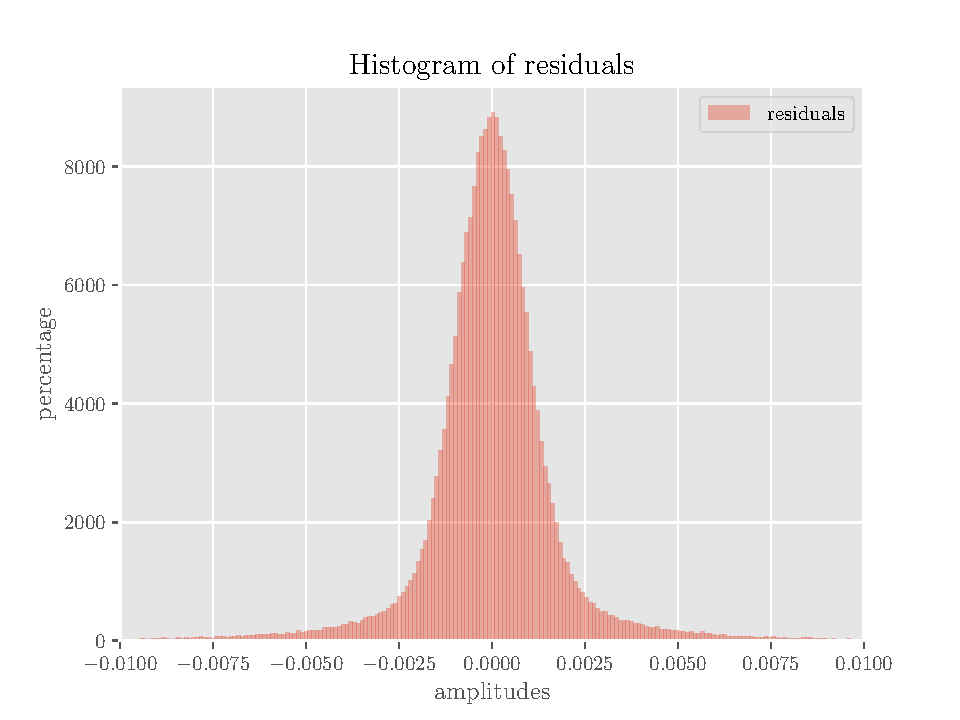
\includegraphics[scale=0.75]{fig_04.pdf}

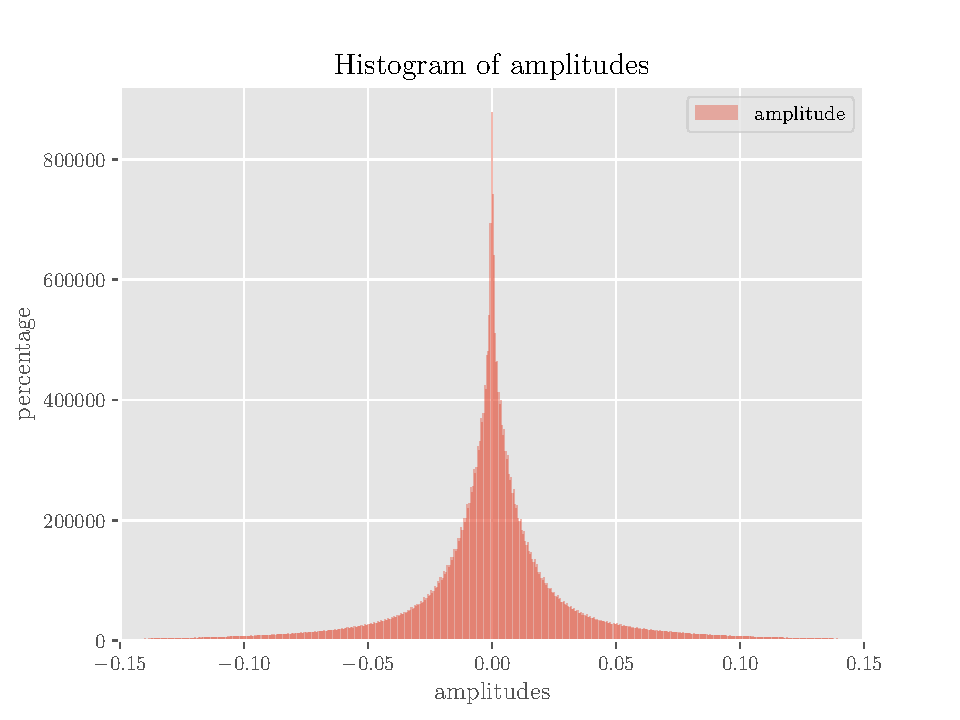
\includegraphics[scale=0.75]{fig_05.pdf}

TODO: add Comments


\section{Question 5}

As a final step, we trained on the whole training set a number of models for $C = 1:20$ and $K = 1:9$. We report our results:

The best Mean Square Error on the training set is achieved with the setting $C=20$ and $K=9$. (As expected, the model with biggest K and C. If not our code should be buggy). For this set up, the Mean square Errors on training, validation and test set are: 
$$MSE_{training} = 7.4563 \cdot 10^{-6}$$
$$MSE_{validation} = 11.1523 \cdot 10^{-6}$$
$$MSE_{testing} = 8.9802 \cdot 10^{-6}$$

The best Mean Square Error on the validation set is achieved with the setting $C=18$ and $K=5$. For this set up, the Mean square Errors on training, validation and test set are: 
$$MSE_{training} = 7.5316 \cdot 10^{-6}$$
$$MSE_{validation} = 7.6156 \cdot 10^{-6}$$
$$MSE_{testing} = 8.0694 \cdot 10^{-6}$$

The best Mean Square Error on the test set is achieved with the setting $C=18$ and $K=4$. For this set up, the Mean square Errors on training, validation and test set are: 
$$MSE_{training} = 7.5556 \cdot 10^{-6}$$
$$MSE_{validation} = 7.6496 \cdot 10^{-6}$$
$$MSE_{testing} = 8.0226 \cdot 10^{-6}$$

So if we were asked to choose the best model, we would respond that it is the $C=18, K=5$ model and its expected mse on future examples will be $E_{gen} = 8.0694 \cdot 10^{-6}$.

\end{document}
